\section{Architecture Design \& Implementation}
\subsection{Overall architecture}

\begin{figure}[htb]
\centerline{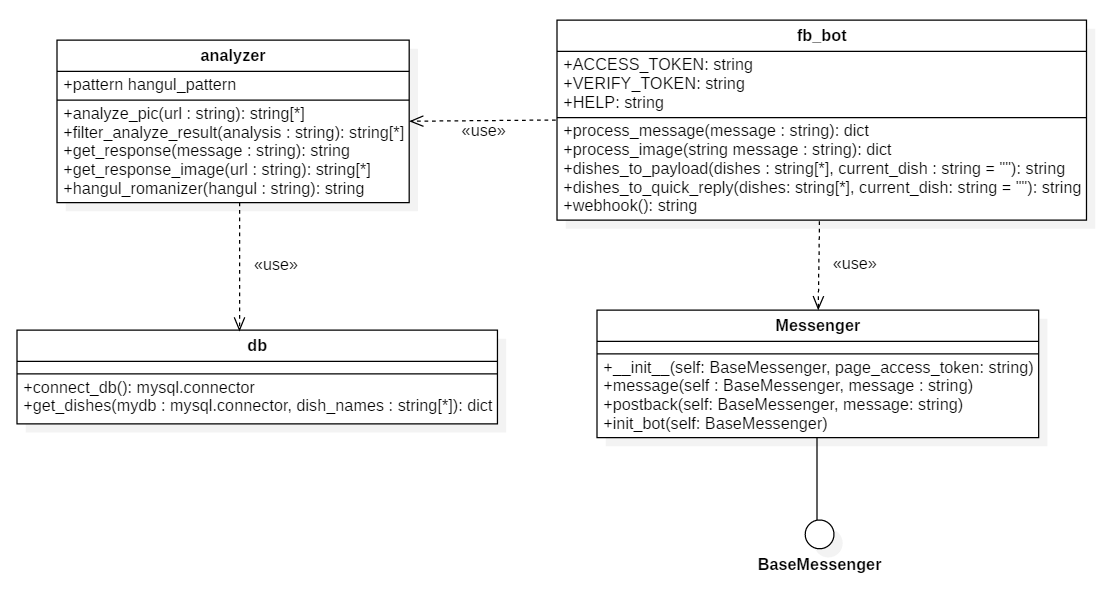
\includegraphics[width=\linewidth]{./pictures/uml}}
\caption{UML of our overall architecture}
\label{fig:uml}
\end{figure}
\FloatBarrier

\subsection{Directory organization}

\begin{table}[htbp]
\caption{Directory organization}
\begin{tabularx}{\linewidth}{|X|X|X|}
\toprule
Directory & File names & Module names in use  \\
\midrule
./src & messenger.py & messenger  \newline\\
./src & fb\_bot.py &  fb\_bot\newline \\
./src & ssl\_certificate.pem db.py \newline  & db \\
./src & analyzer.py & analyzer \newline \\
./tests & 
test.txt \newline 
test\_db.py \newline
test\_json.py	 \newline
test.jpg  \newline
& test\\
./db & food.mwb \newline & db model  \\
./doc & before\_order.tex before\_order.pdf \newline & documentation  \\
./doc/content & architecture\_design\_a nd\_implementation.tex development\_environ ment.tex introduction.tex requirements.tex specifications.tex \newline & documentation \\
./doc/pictures & 
facebook\_dish\_info.png \newline
facebook\_friends.png \newline
facebook\_meun.png \newline
facebook\_message.png \newline
facebook\_overview.png \newline
facebook\_profil.png \newline
facebook\_response.png \newline
facebook\_response\_sele ction.png	\newline
uml.png \newline
class\_uml.mdj 
& documentation \\
\end{tabularx}
\end{table}
\FloatBarrier

\subsubsection{Module 1 - messenger} 

\begin{itemize}

\item Purpose:

The Facebook Messenger chatbot needs Facebook Messenger API to interact with the facebook users who need our service. This module can provides a connection with the Facebook Messenger API, so chatbot can send message to users and receive message from users through this module. It is the most important factor that allows the messenger to function.  

\item Functionality:

This module makes chatbot be able to send messages to the users and receive messages from the users. There is a Facebook server between users and our chatbot server. Facebook provides a webhook function and it gives our chatbot server alerts that user sent a message to our chatbot or other user reaction to our chatbot (entering chatbot chatroom etc.) and messages. Through this module, we can give a response to users immediately and can provide our service. When users send messages, we can implement the appropriate chatbot action and build scenarios in which to communicate with users. It also provides the transmission of text as well as other extension files, such as pictures and files, to enable context-sensitive types of messages to be sent. 

\item Location of Source Code:

/project/src

\item Class component:

The message module has message class. It extends BaseMessenger class, that is provided from the fbmessenger package. fbmessenger is a python library to communicate with the Facebook Messenger API's. It provides various functionality and class to implement the chatbot service. 

\end{itemize}

\subsubsection{Module 2 - fb\_bot}

\subsubsection{Module 3 - analyzer}

\subsubsection{Module 4 - db}

